\documentclass{beamer}
\usetheme{Singapore}
\useoutertheme{miniframes}
\usepackage{etoolbox}
\usepackage{color}
\usepackage[absolute,overlay]{textpos}
\usepackage{graphicx}
\usepackage{ragged2e}

\setbeamertemplate{frametitle}[default][left]

% a flag that tells us how the circles should be drawn
\newif\ifnavbeforecurrent
% reset the flag before every navigation bar
\pretocmd\insertnavigation{\navbeforecurrenttrue}{}{}

% change the circle drawing code so that it changes based on the flag
\defbeamertemplate*{mini frame in current subsection}{changing}[1][50]
{%
  \begin{pgfpicture}{0pt}{0pt}{0.1cm}{0.1cm}
    \pgfpathcircle{\pgfpoint{0.05cm}{0.05cm}}{0.05cm}
    \ifnavbeforecurrent
        \pgfusepath{fill,stroke}
    \else
        \pgfusepath{stroke}
    \fi
  \end{pgfpicture}%
}
\setbeamertemplate{mini frame in current subsection}[changing]

% after the circle for the current frame is drawn, change the flag
\defbeamertemplate*{mini frame}{changing}
{%
  \begin{pgfpicture}{0pt}{0pt}{0.1cm}{0.1cm}
    \pgfpathcircle{\pgfpoint{0.05cm}{0.05cm}}{0.05cm}
    \pgfusepath{fill,stroke}
  \end{pgfpicture}%
  \global\navbeforecurrentfalse
}
\setbeamertemplate{mini frame}[changing]

%%%%%%%%%%%%%%%%%%%%%%%%%%%%%%%%%%%%%%%%%%%%%%%%%%%%%%%%%%%%%%%%%%%%%%%%

\begin{document}


\begin{frame}%Logo Page
\begin{textblock*}{5cm}(3.9cm,0cm)
	\begin{figure}[!h]
	
\includegraphics[width=2cm,height=3cm,keepaspectratio]{images/Logo.png}
	\centering
	\label{fig:Logo}
	\end{figure}
\end{textblock*}

\begin{textblock*}{5cm}(4.7cm,2.7cm)
\textbf{\small University of L'Aquila}
\end{textblock*}

\begin{textblock*}{10cm}(3.1cm,3.2cm)
\textbf{\scriptsize DEPARTMENT OF ENGINEERING COMPUTER}
\end{textblock*}

\begin{textblock*}{10cm}(4.3cm,3.5cm)
\textbf{\scriptsize SCIENCE AND MATHEMATICS}
\end{textblock*}

\begin{textblock*}{10cm}(2.6cm,3.8cm)
\textbf{\scriptsize Master degree in Software Engineering for Adaptive Systems}
\end{textblock*}

\begin{textblock*}{9cm}(2.0cm,4.4cm)
\begin{center}
\textbf{\scriptsize AUTOMATED APPROACHES TO ASSESS THE SIMILARITY
OF OPEN SOURCE PROJECTS}
\end{center}
\end{textblock*}

\begin{textblock*}{2cm}(0.6cm,7.0cm)
\scriptsize Thesis Advisor:
\end{textblock*}
\begin{textblock*}{5cm}(0.6cm,7.3cm)
\textbf{\scriptsize Davide Di Ruscio}
\end{textblock*}

\begin{textblock*}{2.5cm}(9.6cm,7.0cm)
\scriptsize Thesis Co-Advisor:
\end{textblock*}
\begin{textblock*}{5cm}(9.6cm,7.3cm)
\textbf{\scriptsize Phuong T. Nguyen}
\end{textblock*}

\begin{textblock*}{2.5cm}(5.5cm,8.0cm)
\scriptsize Candidate:
\end{textblock*}
\begin{textblock*}{5cm}(5.5cm,8.3cm)
\textbf{\scriptsize Riccardo Rubei}
\end{textblock*}

\end{frame}

\begin{frame}{Table of Contents}%Agenda Page

\begin{textblock*}{5.0cm}(1.5cm,2.0cm)
\begin{itemize}
	\item Introduction
	\item CrossMiner
	\item Contribution
	\item Results
	\item Conclusion
\end{itemize}

\end{textblock*}
\end{frame}

\section{Introduction}
\subsection{Introduction}

\begin{frame}{Introduction}{Challenges}

\begin{itemize}
	\item Searching for canditate components.
	\item Evaluating a set of retrieved canditate components to find the most suitable one.
	\item Adapting the selected components to fit the spicific requirements.
\end{itemize}

\end{frame}

\begin{frame}{Introduction}{CROSSMINER}
\begin{itemize}
	\item CROSSMINER aims at addressing such challenges by providing
	advanced techniques and tools supporting the identification
	and adoption of existing high-quality open source software 
	components instead of implementing in-house propietary solutions
	with similar functionalities.
\end{itemize}

\end{frame}

\begin{frame}{Introduction}{CROSSMINER}
	\begin{figure}[!h]
	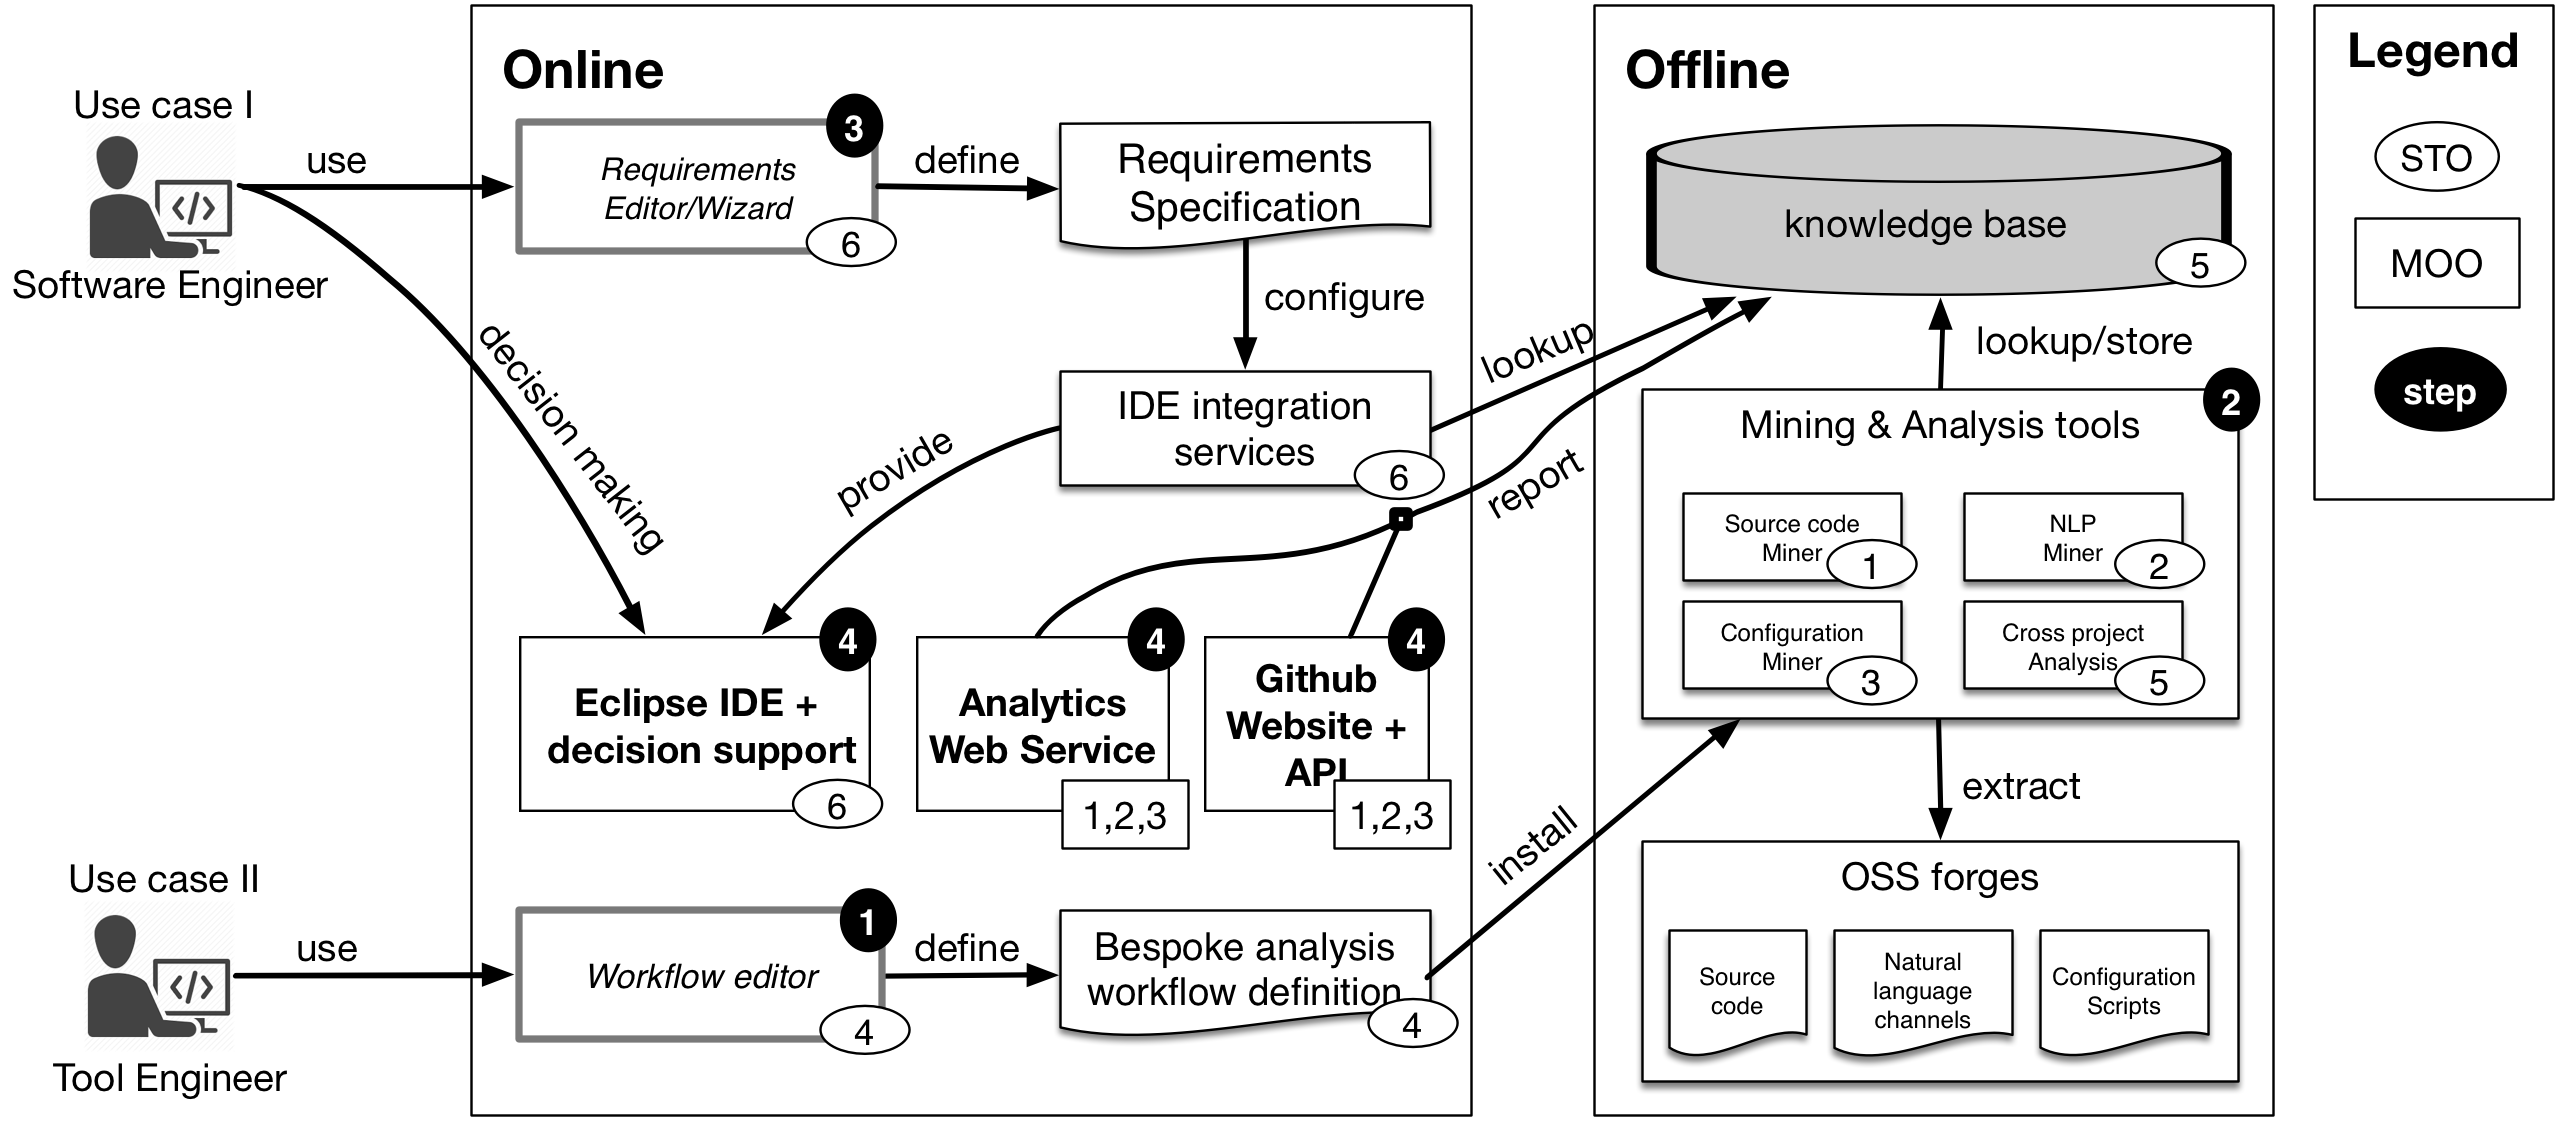
\includegraphics[width=9cm,height=13.5cm,keepaspectratio]{images/crossminer.png}
	\centering
	\label{fig:Crossminer}
	\end{figure}
\end{frame}

\begin{frame}{Introduction}{CROSSMINER}
	\begin{figure}[!h]
	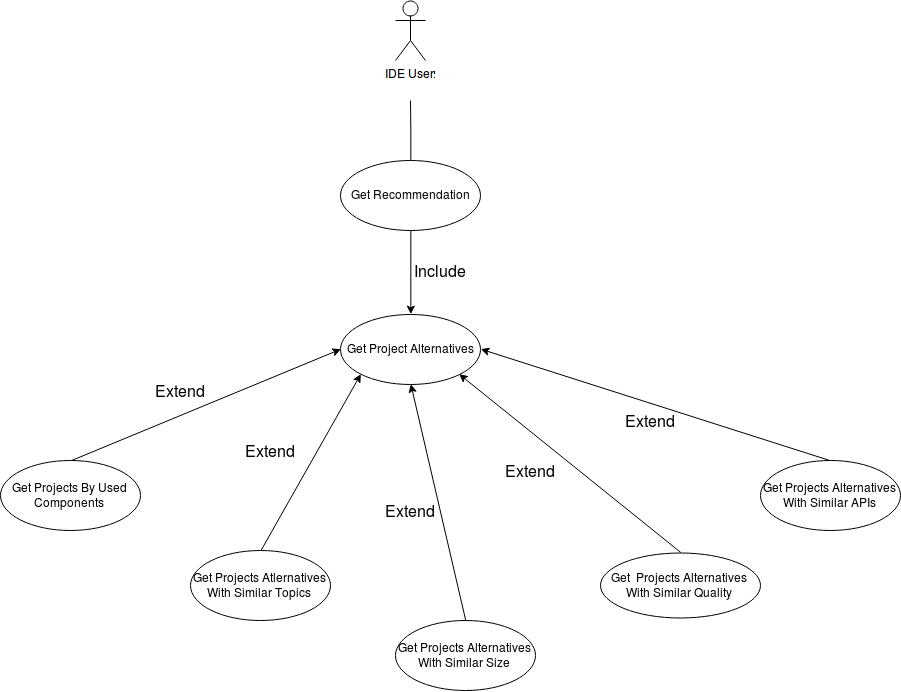
\includegraphics[width=9cm,height=13.5cm,keepaspectratio]{images/UseCaseDiagram.png}
	\centering
	\label{fig:UseCaseDiagram}
	\end{figure}
\end{frame}

\begin{frame}{Introduction}{CROSSMINER}
	\begin{figure}[!h]
	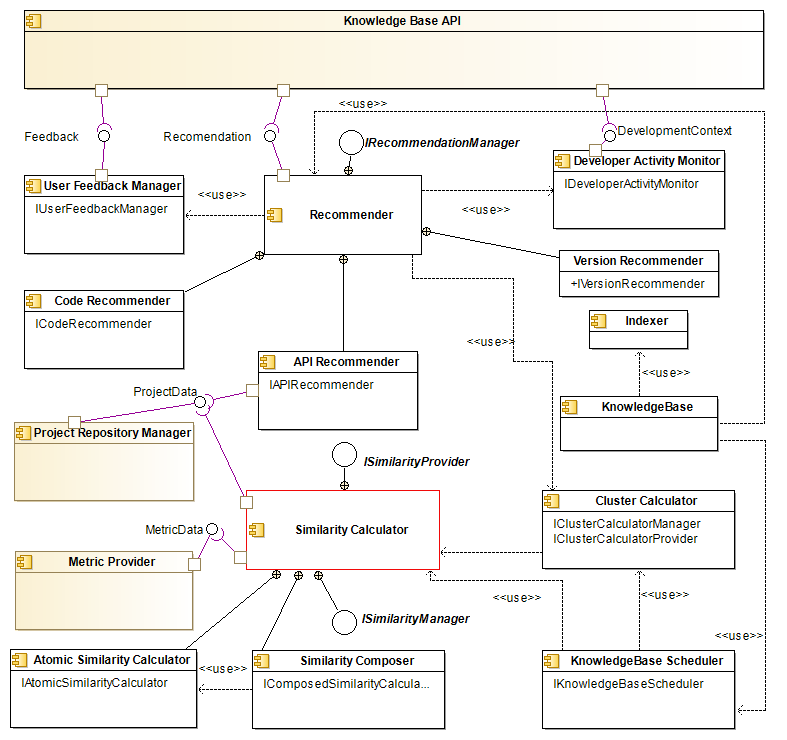
\includegraphics[width=8cm,height=11.5cm,keepaspectratio]{images/component.png}
	\centering
	\label{fig:ComponentDiagram}
	\end{figure}
\end{frame}

\section{Contribution}
\subsection{Contribution}

\begin{frame}{Contribution}{MudaBlue}
	\begin{figure}[!h]
	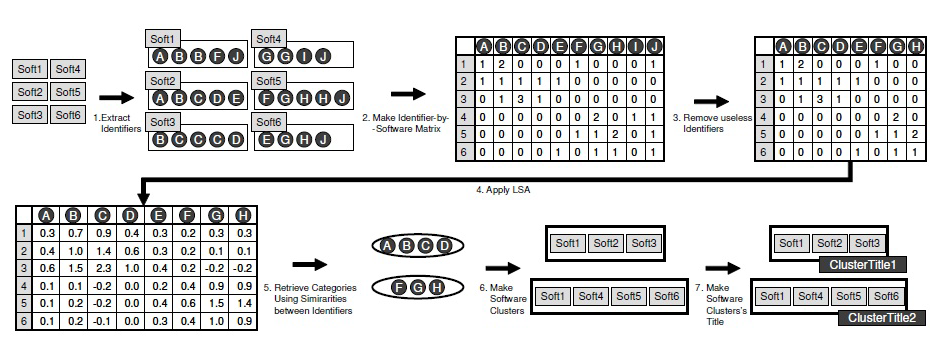
\includegraphics[width=9cm,height=13.5cm,keepaspectratio]{images/Mudablue1.png}
	\centering
	\label{fig:MudaBlue}
	\end{figure}
\end{frame}

\begin{frame}{Contribution}{CLAN}
	\begin{figure}[!h]
	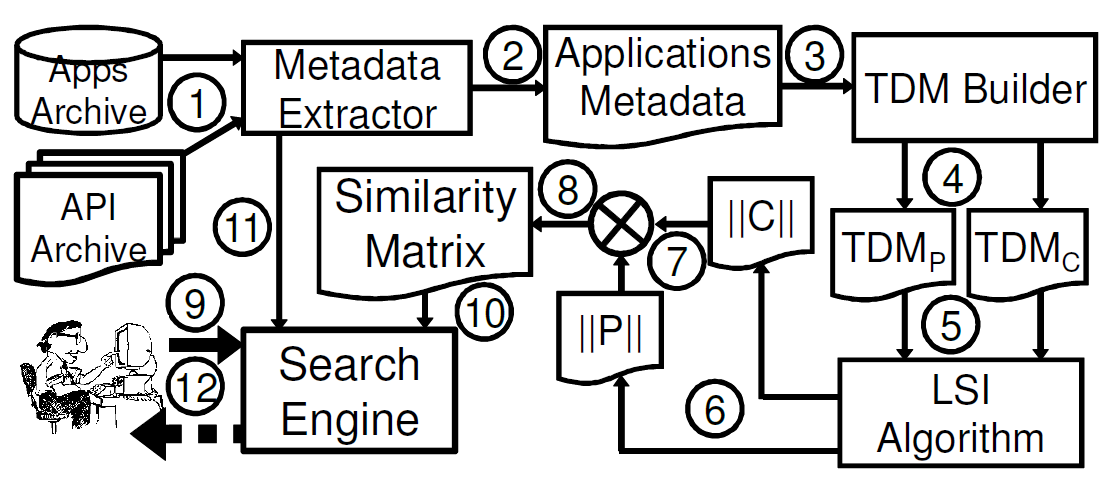
\includegraphics[width=9cm,height=13.5cm,keepaspectratio]{images/Clan.png}
	\centering
	\label{fig:Clan}
	\end{figure}
\end{frame}

\begin{frame}{Contribution}{CROSSSIM}
	\begin{figure}[!h]
	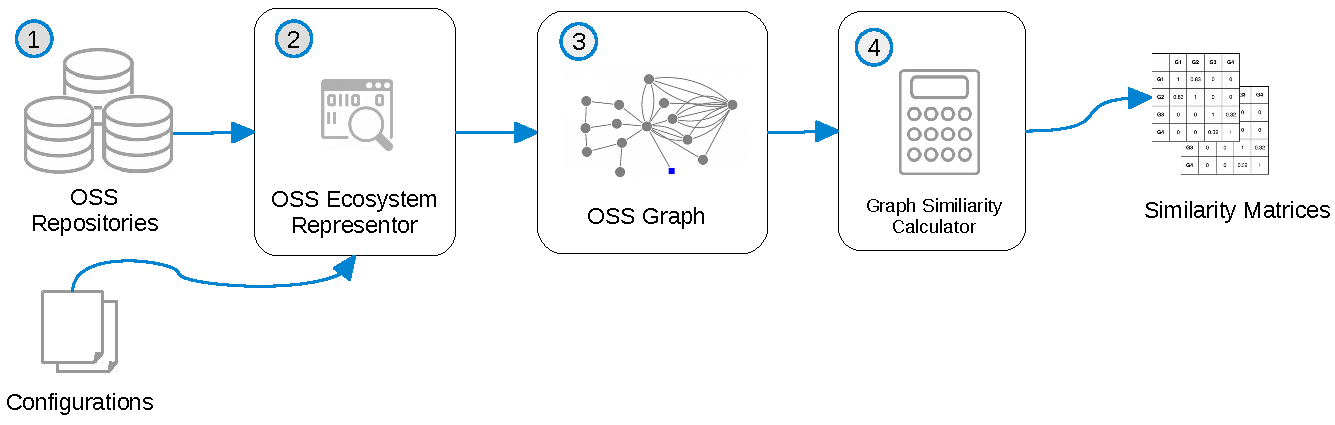
\includegraphics[width=9cm,height=13.5cm,keepaspectratio]{images/CrossSim.pdf}
	\centering
	\label{fig:CrossSim}
	\end{figure}
\end{frame}

\section{Evaluation}
\subsection{Evaluation}

\begin{frame}{Evaluation}{Evaluation Process}
	\begin{figure}[!h]
	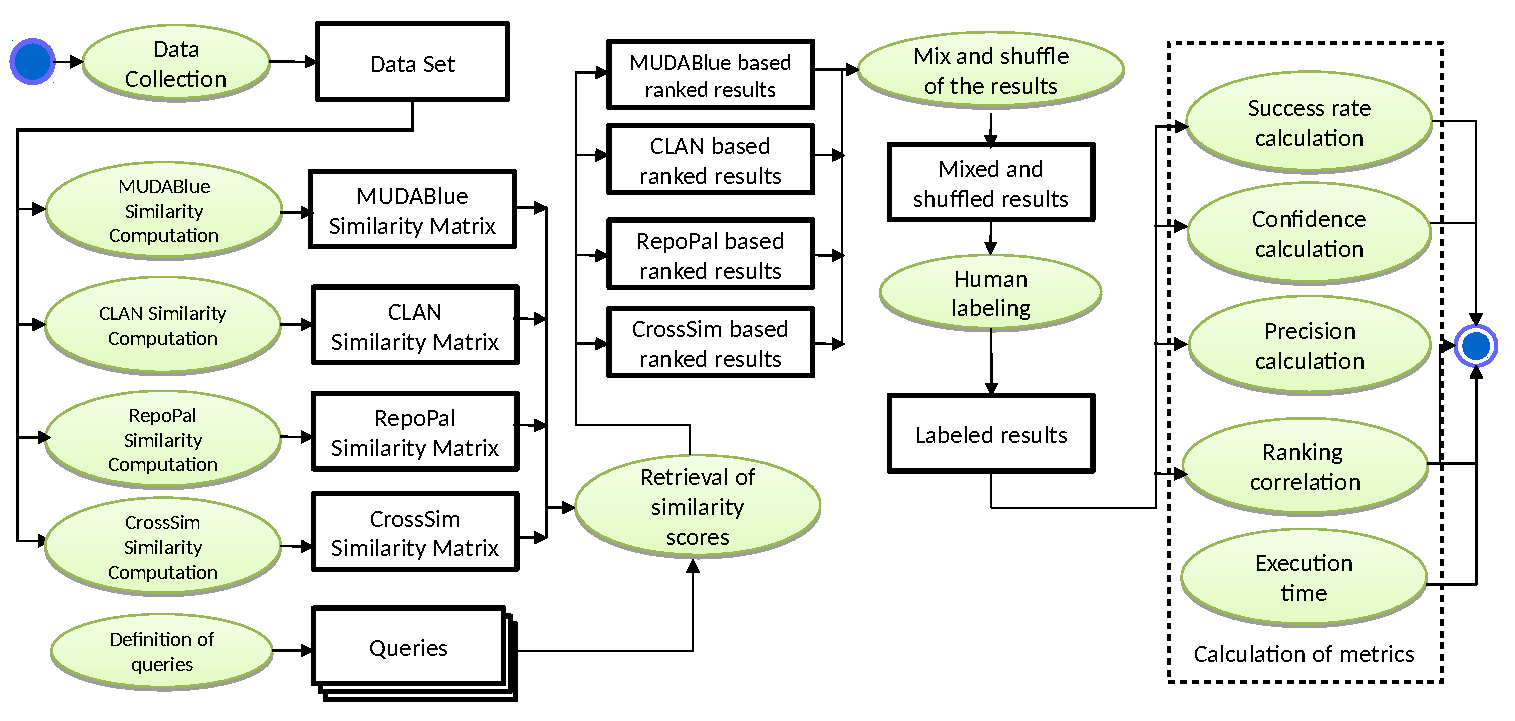
\includegraphics[width=9cm,height=13.5cm,keepaspectratio]{images/EvaluationProcess.pdf}
	\centering
	\label{fig:EvalProcess}
	\end{figure}
\end{frame}

\begin{frame}{Evaluation}{User Study}
	\begin{itemize}
	\item User study: Human evaluators label the similarity between query and retrieved projects
	\item User study: 10 people involved with experience plus a double check
	\item Similarity scales: \emph{Dissimilar}, \emph{Neutral}, \emph{Similar}, and \emph{Highly Similar}
	\item Evaluation metrics: Success Rate, Confidence, Precision
	\end{itemize}
\end{frame}

\begin{frame}{Evaluation}{Results}
\begin{figure}[!tbp]
  \centering
  \begin{minipage}[b]{0.45\textwidth}
    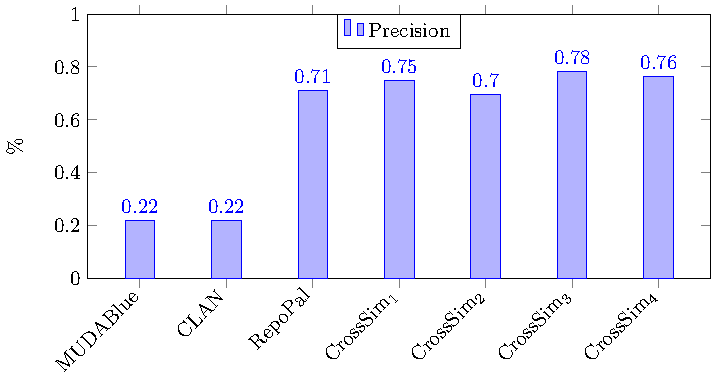
\includegraphics[width=\textwidth]{images/Precision.pdf}
  \end{minipage}
  \hfill
  \begin{minipage}[b]{0.45\textwidth}
    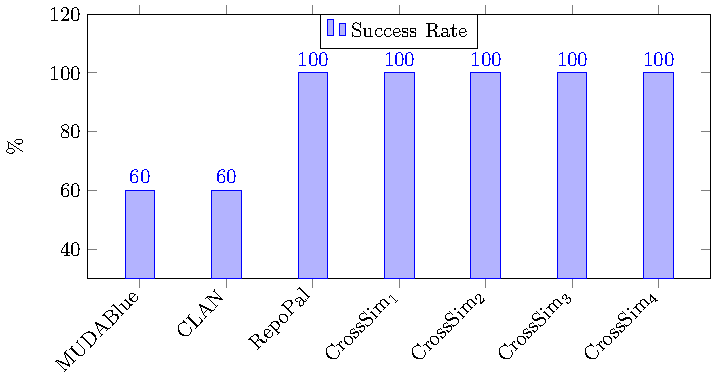
\includegraphics[width=\textwidth]{images/SuccessRate.pdf}
  \end{minipage}
\end{figure}
\end{frame}

\begin{frame}{Evaluation}{Results}
\begin{figure}[!tbp]
  \centering
  \begin{minipage}[b]{0.45\textwidth}
    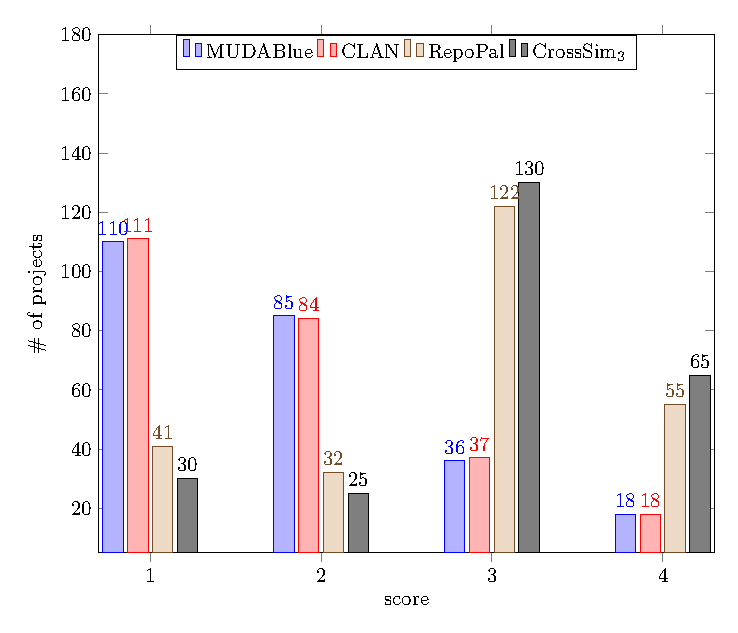
\includegraphics[width=\textwidth]{images/Confidence.pdf}
  \end{minipage}
  \hfill
  \begin{minipage}[b]{0.40\textwidth}
    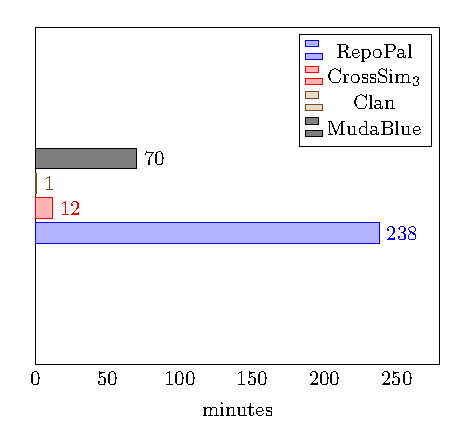
\includegraphics[width=\textwidth]{images/ExecutionTime.pdf}
  \end{minipage}
\end{figure}
\end{frame}

\section{Conclusion}
\subsection{Conclusion}

\begin{frame}{Conclusion}{What Has Been Done}
	\begin{itemize}
		\item Implementation of two approaches
		\item Evaluating the results
		\item Confirmation of the goodness of CrossSim
	\end{itemize}
\end{frame}

\begin{frame}{Conclusion}{What Else to be Done}
	\begin{itemize}
		\item Still much to do
		\item Integrate CrossSime inside the system
		\item Provide Api recommandation
		\item Provide Snippet of Code
	\end{itemize}
\end{frame}

\end{document}
